\ifx \globalmark \undefined %% This is default.
	\documentclass[twoside,openright,11pt,a4paper]{report}

%\compiler avec xelatex
%\usepackage[applemac]{inputenc}
\usepackage[T1]{fontenc}
\usepackage[utf8]{inputenc} %latin1 est possible
%\usepackage[latin1]{inputenc} %latin1 est possible
\usepackage[UKenglish]{babel}
\usepackage{lettrine}

%\usepackage[text={13cm,20cm},centering]{geometry}
\usepackage [squaren, Gray, mediumqspace]{SIunits}
\usepackage [top=2cm, bottom=2cm, left=2cm, right=2cm ]{geometry}

\renewcommand{\familydefault}{cmss}
\addto\captionsenglish{ \renewcommand\chaptername{Solutions of Chapte}}

\usepackage{graphicx}
\usepackage{amsmath}
\usepackage{amsfonts}
\usepackage{amssymb}
\usepackage{amsthm}
\usepackage{bm}
\usepackage{color}

\newcommand{\real}{\mathbb{R}}
\newcommand{\mb}{\mathbf}
\newcommand{\bos}{\boldsymbol}

\def \RR {I \! \! R}

\newcommand{\e}{\begin{equation}}  
\newcommand{\ee}{\end{equation}}
\newcommand{\eqn}{\begin{eqnarray}} 
\newcommand{\eeqn}{\end{eqnarray}} 
\newcommand{\eqnn}{\begin{eqnarray*}} 
\newcommand{\eeqnn}{\end{eqnarray*}} 

\newcommand{\bpm}{\begin{pmatrix}}
\newcommand{\epm}{\end{pmatrix}}

%\newcommand{\{\c c}}{\c c}

\newcommand{\bma}{\left(\begin{array}}
\newcommand{\ema}{\end{array}\right)} 
\newcommand{\hh}{\hspace{2mm}}
\newcommand{\hd}{\hspace{5mm}}
\newcommand{\hu}{\hspace{1cm}}
\newcommand{\vv}{\vspace{2mm}}
\newcommand{\vd}{\vspace{5mm}}
\newcommand{\vm}{\vspace{-2mm}}
\newcommand{\teq}{\triangleq}
%\newcommand{\qedb}{\,$\Box$}
\newcommand{\blanc}{$\left. \right.$}
\newcommand{\frts}[2]%
         {\frac{{\textstyle #1}}{{\textstyle #2}}}

\newcommand{\bindex}[3]%
{
\renewcommand{\arraystretch}{0.5}
\begin{array}[t]{c}
#1\\
{\scriptstyle #2}\\
{\scriptstyle #3}
\end{array}
\renewcommand{\arraystretch}{1}
}

\theoremstyle{definition}
\newtheorem{exemple}{{\bf Exemple}}[chapter]
\newtheorem{theoreme}[exemple]{{\bf Th{é}or{è}me}}
\newtheorem{propriete}[exemple]{{\bf Propri{é}t{é}}}
\newtheorem{definition}[exemple]{{\bf D{é}finition}}
\newtheorem{remarque}[exemple]{{\bf Remarque}}
\newtheorem{remarques}[exemple]{{\bf Remarques}}
\newtheorem{lemme}[exemple]{{\bf Lemme}}
\newtheorem{hypothese}[exemple]{{\bf Hypoth{è}se}}
\newtheorem{exercice}{{\bf Exercice}}[chapter]

\newcommand{\xqedhere}[2]{%
 \rlap{\hbox to#1{\hfil\llap{\ensuremath{#2}}}}}

\newcommand{\xqed}[1]{%
 \leavevmode\unskip\penalty9999 \hbox{}\nobreak\hfill
 \quad\hbox{\ensuremath{#1}}}

\newcommand{\gf}{\fg\,\,}

\newcommand{\cata}[1] %
     {\renewcommand{\arraystretch}{0.5}
     \begin{array}[t]{c} \longrightarrow \\ {#1} \end{array}
     \renewcommand{\arraystretch}{1}}

\usepackage[isu]{caption}
%\usepackage[font=small,format=plain,labelfont=bf,up,textfont=it,up]{caption}
\setlength{\captionmargin}{60pt}

\newcommand{\cqfd}
{%
\mbox{}%
\nolinebreak%
\hfill%
\rule{2mm}{2mm}%
\medbreak%
\par%
}

\pagestyle{headings}

\renewcommand{\sectionmark}[1]{%
\markright{\thesection.\ #1}{}}

\renewcommand{\chaptermark}[1]{%
\markboth{\chaptername\ \thechapter.\ #1}{}}

\makeatletter 
\def\@seccntformat#1{\csname the#1\endcsname.\;} 
\makeatother

\title{ {\Huge {\textbf{Modélisation et analyse  \\ \vspace{4mm} des systèmes dynamiques }}} \\ \vspace{4cm} G. Bastin}

%\title{ {\Huge {\textbf{Modelisation et analyse  \\ \vspace{4mm} des systemes dynamiques }}} \\ \vspace{4cm} G. Bastin}


\date{\today}
	\begin{document} %% Crashes if put after (one of the many mysteries of LaTeX?).
\else 
	\documentclass{standalone}
	\begin{document}
\fi

\graphicspath{ {Chapitre5/images/} }	

\setcounter{chapter}{4}
\chapter{Systèmes réactionnels}
\chaptermark{Systèmes réactionnels}\label{sysreac}	
	
\lettrine[lines=1]{\bf L}{}a notion de système réactionnel recouvre une classe de systèmes
dynamiques utilisés dans des domaines variés des sciences de l'ingénieur 
tels que le génie
chimique, le génie biomédical, les biotechnologies ou l'écologie. Sous une
hypothèse générale d'homogénéité spatiale, la  dynamique des systèmes
réactionnels est décrite par des équations différentielles de bilan. Ces
équations sont obtenues par la combinaison d'un {\em réseau réactionnel}
qui encode les réactions qui sont supposées se dérouler dans le système 
avec deux phénomènes physiques de base : les {\em cinétiques de
réaction} d'une part et les {\em dynamiques d'échange} d'autre part. Ces
divers éléments de la description des systèmes réactionnels seront
présentés dans les sections qui vont suivre en  commen\c cant par les
réseaux réactionnels.

\section{Réseaux réactionnels}

Un système réactionnel est caractérisé par un certain nombre de {\em
réactions}  entre des {\em espèces} de nature chimique ou biologique. Les
espèces sont en nombre fini $n$ et nous les désignons par
les symboles suivants : 
\eqnn 
X_1, X_2, X_3,  \ldots , X_n.
\eeqnn 
Les réactions sont
elles aussi en nombre fini $m$ et se déroulent à l'intérieur d'un domaine
géométriquement bien délimité. Par exemple un réacteur chimique s'il
s'agit de réactions entre espèces chimiques, ou encore une niche
écologique s'il s'agit d'interactions entre espèces animales. La frontière du
domaine est elle aussi bien délimitée et elle sépare le système du monde
extérieur. 

Pour présenter la notion de réseau réactionnel, le plus simple est de
commencer par un exemple.

\begin{exemple} {\bf Réaction chimique}

Le mécanisme de la réaction entre l'oxyde nitrique et l'hydrogène est
décrit par le réseau réactionnel suivant qui comprend $m=4$ réactions
mettant en oeuvre $n=6$ espèces chimiques : 
\eqn 
2X_1 &\longrightarrow& X_2 \label{oxnit1}\\ 
X_2 &\longrightarrow& 2X_1 \\ 
X_2 + X_3&\longrightarrow& X_4 + X_5 \\ 
X_3 + X_5 &\longrightarrow& 2X_6 \label{oxnit4}  
\eeqn 
Les six espèces sont~: $X_1 = NO$, $X_2 = N_2O_2$, $X_3 = H_2$, $X_4 = N_2$,
$X_5 = H_2O_2$, $X_6 = H_2O$.   \qed
\end{exemple}

Un réseau réactionnel est donc un ensemble de $m$ réactions de la forme
suivante : 
\eqnn 
\sum_{i=1}^n\gamma_{ij}X_i \longrightarrow
\sum_{i=1}^n\delta_{ij}X_i  \hspace{5mm} j=1,\ldots,m \hspace{5mm}
\gamma_{ij} \geq 0 \hspace{5mm} \delta_{ij} \geq 0.
\eeqnn 
Les coefficients
$\gamma_{ij}$ et $\delta_{ij}$ sont des nombres réels positifs appelés {\em
coefficients stoechiométriques}. Ils expriment la quantité nominale de
l'espèce $X_i$ qui est consommée ou produite par la $j$-ième réaction.
Par exemple, la quatrième réaction du réseau ci-dessus signifie : une
mole de $X_3$ combinée à une mole de  $X_5$  produit deux moles de
$X_6$. 

Nous introduisons les notations matricielles suivantes~:
\begin{equation*} \begin{split}
\Gamma &= [\gamma_{ij}] \hh \hh \mbox{matrice } n \times m \text{ avec éléments } \gamma_{ij} \\
\Delta &= [\delta_{ij}] \hh \hh \mbox{matrice } n \times m \text{ avec éléments } \delta_{ij}
\end{split} \end{equation*}
La {\em matrice stoechiométrique} est définie comme suit~:
\begin{equation*} \begin{split}
C = \Delta - \Gamma.
\end{split} \end{equation*}
Le rang $p$ de cette matrice est appelé {\em rang du
réseau réactionnel}. Il désigne le nombre de réactions indépendantes.

Par convention, toutes les réactions s'écrivent avec une flèche allant de
la gauche vers  la droite. Ainsi dans l'exemple ci-dessus, la  réaction {\em
réversible} $2X_1 \leftrightarrows X_2$ est encodée sous la forme de deux
réactions simples distinctes : 
\eqnn 
2X_1 &\longrightarrow& X_2 \\ X_2
&\longrightarrow& 2X_1 
\eeqnn

\subsection* {Réactifs et produits}

Les {\em réactifs} sont les espèces $X_i$ qui apparaissent du c\^oté
gauche  des réactions avec un coefficient $\gamma_{ij} > 0$.

Les {\em produits} sont les espèces $X_i$ qui apparaissent du c\^oté droit
des réactions et avec un coefficient $\delta_{ij} > 0$. 

Une espèce $X_i$ peut être à la fois réactif dans une réaction et un
produit dans la même ou dans une autre  réaction. C'est le cas de l'espèce $X_5$ dans l'exemple 5.1.

Un {\em produit terminal} est une espèce produite par une réaction au
moins mais qui n'est  réactif d'aucune réaction.

Un {\em réactif initial} est une espèce consommée par une réaction au
moins mais qui n'est  produite par aucune réaction. 

A titre d'exemple, dans le réseau réactionnel (\ref{oxnit1}) - (\ref{oxnit4}),
on peut identifier les sous-ensembles suivants : 
\begin{itemize} 
\item[] Réactifs : $X_1, X_2, X_3, X_5$ 
\item[] Produits : $X_1, X_2, X_4, X_5, X_6$ 
\item[] Réactifs initiaux : $X_3$ 
\item[] Produits terminaux : $X_4, X_6$ 
\end{itemize} 

\subsection* {Catalyseurs et autocatalyseurs}

Comme nous venons de l'indiquer, une espèce donnée peut apparaître
des deux côtés d'une même réaction. C'est par exemple le cas de
l'espèce $X_2$ dans la réaction suivante : \eqnn \gamma_1X_1 + \gamma_2X_2
\longrightarrow \delta_2X_2 + \delta_3X_3 \eeqnn Si $\gamma_2 = \delta_2$,
l'espèce $X_2$ est un {\em catalyseur}, c'est à dire une espèce  qui n'est ni
consommée, ni produite mais dont la présence est indispensable pour que la
réaction ait lieu.

Si $\gamma_2 < \delta_2$, l'espèce $X_2$ est un {\em autocatalyseur},
c'est à dire une espèce  qui est un catalyseur de sa propre production.

Pour les réactions catalytiques et autocatalytiques, on utilise aussi une
représentation  alternative qui consiste à ne pas faire figurer le catalyseur
à gauche de la réaction, mais à l'indiquer sous la flèche sans coefficient
et à le pondérer à droite avec le coefficient $\delta_2 - \gamma_2$ : \eqnn
\gamma_1X_1  \cata{X_2} (\delta_2 - \gamma_2)X_2 + \delta_3X_3 \eeqnn Parmi
les exemples les plus typiques de réactions autocatalytiques on peut citer
 les réactions de polymérisation ou encore les réactions de croissance
microbienne comme dans l'exemple ci dessous.

\begin{exemple} {\bf \em Fermentation alcoolique}

Le mécanisme sous-jacent aux fermentations alcooliques peut
être décrit par le réseau réactionnel suivant : \eqnn X_1 + 2.33X_2 +
0.525X_3 &\cata{X_4}& 3.5X_4 + 2.5X_5 + 3.66X_6 \nonumber \\ X_1 +
0.054X_3 &\cata{X_4}& 0.36X_4 + 1.89X_5 + 0.14X_6 + 1.88X_7 \nonumber \\
1.61X_2 + 0.193X_3 + X_7 &\cata{X_4}& 1.32X_4 + 0.68X_5 + 2.12X_6
\nonumber \eeqnn Les sept espèces sont : glucose $X_1$, oxygène $X_2$,
ammoniaque $X_3$, levures $X_4$,  dioxide de carbone $X_5$, eau $X_6$,
éthanol $X_7$.  \qed
\end{exemple}

\section{Modèle d'état des systèmes réactionnels}

La présence de chacune des espèces à l'intérieur du système peut être
quantifiée.  On note $x_i(t)$ la quantité de l'espèce $X_i$ par unité de
volume dans le système. Le vecteur des concentrations, qui sera aussi le
vecteur d'état du  modèle est noté~: 
$$
x(t) \teq (x_1(t), x_2(t), \cdots , x_n(t))^T.
$$

Les vitesses de réaction, aussi appelées {\em cinétiques de réaction},
expriment la vitesse de consommation des réactifs et de formation des
produits par unité de volume dans le système, selon le réseau
réactionnel. Une vitesse de réaction  $r_j$ est associée à chaque
réaction du réseau $(j = 1, \cdots , m)$. Les vitesses de réaction sont fonction des concentrations $x_i$ des différentes espèces, mais aussi éventuellement d'autres facteurs physico-chimiques qui sont en jeu dans le système tels, par exemple, la température ou la lumière. Nous considérons ici le cas particulier où elles ne dépendent que de l'état $x$. Le vecteur des cinétiques
de réaction est noté :  $$  r(x) \teq (r_1(x), r_2(x), \cdots ,
r_m(x))^T.  $$
Chacune des fonctions $r_j :
\mathbb{R}_{+}^{n} \rightarrow \mathbb{R}_{+}$ est à valeurs positives
 et définie sur l'orthant positif. Il est clair qu'une réaction ne peut se
dérouler que si tous les réactifs sont présents en quantité non nulle dans
le système. Autrement dit, la vitesse d'une réaction est nécessairement
nulle si l'un des réactifs de la réaction est absent du système. En termes
mathématiques, cette condition s'exprime comme suit : 
\begin{hypothese} \label{cond}

\eqn 
&& \mbox{1) } r_j(x) \geq 0 \hspace{3mm} \forall j \hspace{3mm} \forall x \in \mathbb{R}_{+}, \label{cond1}\\ 
&& \mbox{2) }  r_j(x) = 0 \mbox{ si } x_i = 0  \mbox{ pour une valeur de } i, 
\in I^{rj} \label{cond2} 
\eeqn
où $I^{rj}$ désigne l'index de l'ensemble des réactifs (y compris les
catalyseurs)
 mis en oeuvre dans la réaction d'indice $j$.  \qed
\end{hypothese}

Sur base de la description des réseaux réactionnels et des vitesses de
réaction, on vérifie alors aisément que le bilan quantitatif de chaque
espèce à l'intérieur du domaine du système s'écrit comme suit~: 
$$
\dot x_i = \sum_{j = 1}^{m} (\delta_{ij} - \gamma_{ij})r_j(x(t)) + \frac{1}{V}(Q_{0i}(t) -
Q_{i0}(t)). \label{contireac}
$$
Dans cette équation, les notations $\delta_{ij}$, $\gamma_{ij}$ (coefficients
stoechiométriques) et $r_j(x(t))$ (vitesses de réaction) ont été
définies plus haut. La notation $V$ désigne le volume (supposé constant) du domaine considéré. Les notations $Q_{0i}(t)$ et $Q_{i0}(t)$ désignent les flux de l'espèce $X_i$ à travers la frontière du domaine~:
\begin{description}
\item $Q_{io}(t)$ désigne le flux circulant du domaine vers l'extérieur,
\item $Q_{oi}(t)$ désigne le flux circulant de l'extérieur vers le
domaine.
\end{description}

Cette équation de continuité exprime
que la variation, par  unité de temps,  de la  concentration de l'espèce $X_i$
résulte de deux mécanismes : 
\begin{itemize}
\item le terme $\sum_{j = 1}^{m} (\delta_{ij} - \gamma_{ij})r_j(x(t))$
exprime la différence, par unité de volume, entre la somme des quantités produites et la somme
des quantités consommées dans les réactions où
cette espèce $X_i$ est respectivement un produit ou un réactif;
\item le terme $Q_{0i}(t) - Q_{i0}(t)$ est la différence entre le flux entrant et
le flux sortant de cette même espèce $X_i$ à travers la frontière du
domaine.
\end{itemize}

On dit que le système est {\em fermé} lorsque
$Q_{io}(t) =  Q_{oi}(t) = 0$ pour tout $i$ et pour tout $t$, c'est à dire lorsqu'il
n'y a aucun échange avec l'extérieur.  Dans le cas contraire, on dit que le
système est {\em ouvert}. 

La mise en équation du modèle d'état d'un système réactionnel
comporte donc trois aspects fondamentaux.

Premièrement, le réseau réactionnel détermine le nombre de variables
d'état ainsi que la structure et la valeur numérique des coefficients de la
matrice stoechiométrique $C$.

Ensuite se pose la question de la modélisation  des
vitesses de réaction $r_j(x)$ en fonction des variables d'état $x_i$. Cette
modélisation fera l'objet de la section suivante.

Il faut enfin modéliser les flux d'entrée et de sortie en fonction des
variables d'état et d'entrée :
\eqnn
Q_{0i}(x,u) \hspace{1cm} Q_{i0}(x,u)
\eeqnn
Cette modélisation sera illustrée par les divers exemples qui seront
considérés ultérieurement.

La dynamique d'un système réactionnel
est alors représentée par le modèle d'état suivant~: 
\eqn 
\dot x =  Cr(x) + q_{in}(x,u) - q_{out}(x,u) \label{sysrea} 
\eeqn
où la définition des vecteurs $q_{in}(x,u)$ et $q_{out}(x,u)$ est évidente. Il est clair que ce
modèle d'état n'a de sens et ne peut donc être défini que dans l'orthant
positif. On montre d'ailleurs facilement que, sous l'hypothèse \ref{cond}, le
système (\ref{sysrea}) est  un système positif qui possède une structure de système à compartiments.

Pour un système fermé, les vecteurs $q_{in}$ et
$q_{out}$ sont identiquement nuls  et le modèle d'état se réduit à
l'équation~:
$$
\dot{x} = Cr(x). \label{sysreaferm}
$$

\begin{hypothese} \label{princon} {\bf \em Principe de conservation}

Le noyau de la matrice stoechiométrique contient un vecteur positif~:
$$
\exists \hh \omega = (\omega_1, \ldots , \omega_n)^T \hh
\omega_i > 0 \hh i=1,\ldots,n \hh \mbox{ tel que } \omega \in \ker C^T. \xqedhere{2cm}{\qed}
$$
\end{hypothese}

Sous cette hypothèse on vérifie aisément que la quantité
$$
z = \sum_{i=1}^m \omega_i x_i = \omega^Tx
$$
est un invariant du système (\ref{sysreaferm}) (c'est-à-dire que $z(t)$
est constante le long des solutions du système). En effet
$$
\dot z = \sum_{i=1}^n \omega_i \dot x_i = [\omega^TC]r(x) = 0 
$$
et la quantité entre crochets est nulle en vertu de l'hypothèse \ref{princon}.

Cette hypothèse est fondamentale car elle exprime en fait que, en accord
avec la réalité physique, un système réactionnel fermé est un système
conservatif en ce sens que la quantité totale contenue dans le système est
constante : les quantités produites compensent exactement les quantités
consommées (moyennant le choix de coefficients de normalisation
$\omega_i$ appropriés) ou, comme disait Lavoisier, \og rien ne se perd, rien
ne se crée \fg.

\section{Modélisation des cinétiques de réactions}

Lorsqu'une réaction obéit au {\em principe d'action des masses}, une
expression  générale classique de fonction cinétique satisfaisant les
conditions (\ref{cond1}) - (\ref{cond2}) est la suivante : 
$$ 
r_j(x) = k_j\prod_{i \in I^{rj}} x_i^{\nu_{ij}} 
$$
où $k_j$ est la {\em constante de vitesse} de la $j$-ième réaction. Le principe d'action des masses consiste donc à exprimer chaque vitesse de réaction comme étant proportionnelle
au produit des concentrations des réactifs de la réaction (y compris les
catalyseurs), chaque concentration étant élevée à la puissance positive
$\nu_{ij}$ appelée {\em ordre} de la $j$-ième réaction par rapport à la
$i$-ième espèce. La {\em loi d'action des  masses} correspond au cas
particulier où $\nu_{ij} = \gamma_{ij} \hh \forall (i,j)$, c'est à dire 
où les ordres de la réaction coïncident avec les coefficients stoechiométriques des 
réactifs.

Il arrive souvent que le principe d'action des masses ne suffise pas à rendre
compte des vitesses de réaction observées expérimentalement. On est
amené alors à généraliser le modèle de la fa\c con suivante : \eqnn r_j(x) = 
k_j\prod_{i \in I^{rj}} \rho_{ij}(x_i) \eeqnn où les fonctions $\rho_{ij} :
\mathbb{R}_{+} \rightarrow \mathbb{R}_{+}$ satisfont les conditions suivantes : \eqnn
&& \rho_{ij}(x_i) \geq 0 \hh \hh \forall x_i \geq 0 \\ && \rho_{ij}(0) = 0 \eeqnn
Souvent, les fonctions $\rho_{ij}(x_i)$ sont monotones croissantes, comme
sur la figure  \ref{Fig:monocrois}. 
\begin{figure}[htbp] 
   \centering
   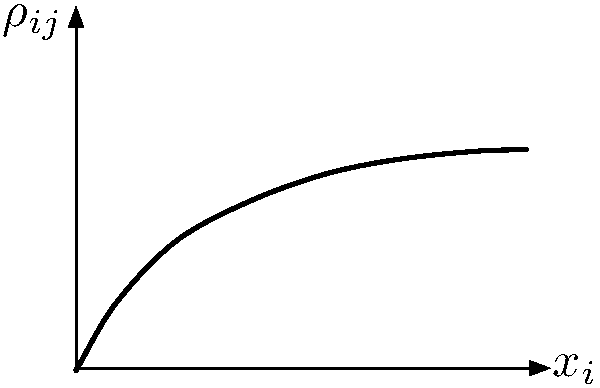
\includegraphics[height=4cm]{monocrois} 
   \caption{Fonction cinétique monotone croissante}
   \label{Fig:monocrois}
\end{figure}
Un des exemples les plus courants est connu
sous le nom de  cinétique de Michaelis-Menten représentée par la fonction
$$ 
\rho_{ij}(x_i) = \frac{x_i}{K_{ij} + x_i}.
$$ 


\subsection*{Inhibiteurs et activateurs}

Il peut arriver qu'une réaction soit ralentie par la présence d'un produit
de la réaction ou d'une autre espèce quelconque apparaissant dans le
réseau réactionnel. Un tel effet {\it inhibiteur} est modélisé en ajoutant un
terme multiplicatif supplémentaire dans le modèle  cinétique. Ce terme est
une fonction décroissante de la concentration du composant inhibiteur. Les
deux modèles suivants sont les plus fréquents~: 
\eqn 
&& \mbox{inhibition hyperbolique : } \rho_{ij}(x_i) = \frac {K_{ij}}{K_{ij} + x_i}, \label{inhibhyper} \\ && \mbox{inhibition exponentielle : } \rho_{ij}(x_i) = e^{-(K_{ij}x_i)}.
\label{inhibexpo} 
\eeqn

\begin{exemple}  Considérons le réseau réactionnel suivant~:
\begin{equation} \begin{split} \label{exa}
X_1 + X_2 \; &\longrightarrow \; 2X_3, \\ 
2X_3 \; &\longrightarrow \; X_4. 
\end{split} \end{equation}
Supposons que les cinétiques obéissent à la loi d'action des
masses et que la première réaction soit de plus 
inhibée par le produit $X_4$ de la
seconde réaction selon une loi  exponentielle (\ref{inhibexpo}). Les deux
cinétiques de réactions auront la forme suivante : 
\begin{equation} \begin{split} \label{cin}
r_1(x) &= k_1x_1x_2e^{-(Kx_4)}, \\
r_2(x) &= k_2x_3^2. \xqedhere{6.2cm}{\qed}
\end{split} \end{equation}
\end{exemple}

Il peut arriver aussi qu'une espèce  quelconque apparaissant dans le schéma 
ait un effet accélérateur sans pour autant être indispensable 
à la réaction
(ce n'est ni un réactif ni un catalyseur de la réaction). Un tel effet {\it activateur} 
est modélisé en ajoutant un
terme multiplicatif supplémentaire dans le modèle  cinétique. Ce terme est
une fonction croissante de la 
concentration du composant activateur {\em qui ne s'annulle pas à l'origine}.

\section{Les réacteurs parfaitement mélangés}

Les réacteurs chimiques ou biologiques parfaitement
mélangés constituent l'un des exemples les
plus typiques de système réactionnel. Ces réacteurs sont constitués d'un
réservoir contenant un milieu réactionnel liquide qui est mélangé en
permanence par un système d'agitation approprié et dont la composition
est homogène. Les différents réactifs peuvent être fournis
au réacteur sous forme liquide ou sous forme gazeuse. Les produits de réaction
sont formés en solution dans le milieu réactionnel. Certains de ces produits
peuvent être facilement gazéïfiables et s'échapper librement du réacteur
sous forme gazeuse. Le milieu réactionnel est soutiré du réacteur en vue de
la récolte des produits.

\subsection {Réacteurs continus}

Un réacteur parfaitement mélangé fonctionne en {\em mode continu} lorsque les
débits d'alimentation et de soutirage sont ajustés de sorte que le volume $V$
du milieu réactionnel soit constant. On parle alors d'un réacteur continu
parfaitement mélangé (acronyme CSTR pour {\em
continuous stirred tank reactor}). Un exemple de réacteur de ce type est
représenté à la figure \ref{Fig:CSTR}. 
\begin{figure}[htbp] 
   \centering
   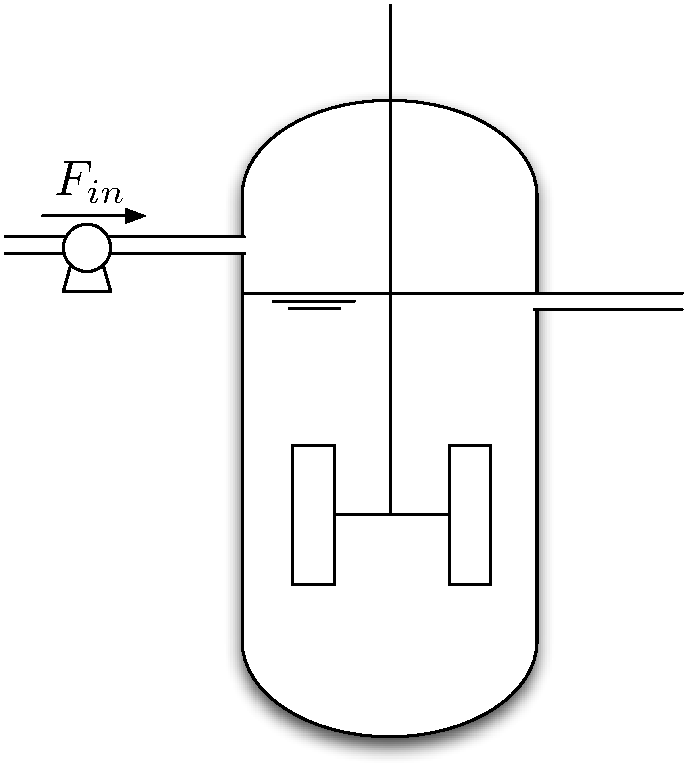
\includegraphics[height=6cm]{CSTR} 
   \caption{Réacteur continu parfaitement mélangé}
   \label{Fig:CSTR}
\end{figure}
Le réservoir est muni d'une canalisation d'alimentation et d'un dispositif de
trop-plein de manière à maintenir le volume constant.

On suppose que ce réacteur est le lieu d'un ensemble de $m$ réactions
impliquant $n$ espèces chimiques $X_1, X_2, \dots , X_n$. Les concentrations
des différentes espèces dans le milieu réactionnel sont notées  $x_i$. Les
diverses espèces sont fournies au réacteur en solution ou en suspension dans
le flux d'alimentation avec des concentrations notées $x_i^{in}$.
Le débit volumétrique d'alimentation est noté $F_{in}$. Avec ces notations et
définitions, les équations de bilan des différentes espèces dans le réacteur
s'écrivent sous la forme matricielle suivante~:
$$
\dot xV = Cr(x)V - F_{in}x + F_{in}x^{in}
$$
où $C$ est la matrice stoechiométrique du réseau réactionnel, $r(x)$ le vecteur
des vitesses de réactions, $x$ le vecteur des concentrations $x_i$ et $x^{in}$ le
vecteur des concentrations d'alimentation $x_i^{in}$.

En définissant la variable
d'entrée
$$ 
u \triangleq \frac{F_{in}}{V}
$$
qui est le débit d'alimentation par unité de volume, appelé aussi {\em taux de
dilution} (l'inverse du taux de dilution est le temps de séjour), on obtient le
modèle d'état d'un réacteur continu parfaitement mélangé~:
$$
\dot x = Cr(x) - ux + ux^{in}. \label{CSTR}
$$
On observe que ce modèle possède la structure (\ref{sysrea}) avec les
définitions suivantes~:
$$
q_{out}(x,u) = ux \hh \hh \hh q_{in}(x,u) = ux^{in}.
$$

\begin{exemple}{\blanc} \label{exempleCSTR}

Nous considérons un réacteur chimique parfaitement mélangé dans lequel
les deux réactions (\ref{exa}) se déroulent simultanément dans la
phase liquide avec les cinétiques (\ref{cin}).     Le réacteur est
alimenté par les deux réactifs initiaux $X_1$ et $X_2$ en solution avec des
concentrations d'alimentation
$x_1^{in}$ et $x_2^{in}$.

Le modèle d'état s'écrit
$$
\bma{c} \dot x_1 \\ \dot x_2 \\ \dot x_3 \\ \dot x_4 \ema =
\bma{cc} -1 & 0 \\ -1 & 0 \\ 2 & -2 \\ 0 & 1 \ema \bma{c}
k_1x_1x_2e^{-(Kx_4)} \\ k_2x_3^2 \ema 
 + u \bma{c} x_1^{in} -x_1 \\ x_2^{in} -x_2 \\ -x_3 \\ -x_4
\ema   
$$
où les variables d'état $x_1, x_2, x_3$ et $x_4$ représentent les
concentrations des différentes espèces dans le milieu réactionnel. \qed
\end{exemple}

\subsection{Réacteurs à volume variable}

Considérons maintenant le réacteur représenté à la figure \ref{Fig:CSTR2}. Il est
identique au précédent sauf que le trop-plein est remplacé par une canalisation
de soutirage dont le débit volumétrique $F_{out}$ est contrôlé par
une pompe. Dans le cas particulier où ce débit $F_{out}$ peut être nul par
intermittence (pas de soutirage), on dit que le réacteur fonctionne en mode
discontinu.
\begin{figure}[htbp] 
   \centering
   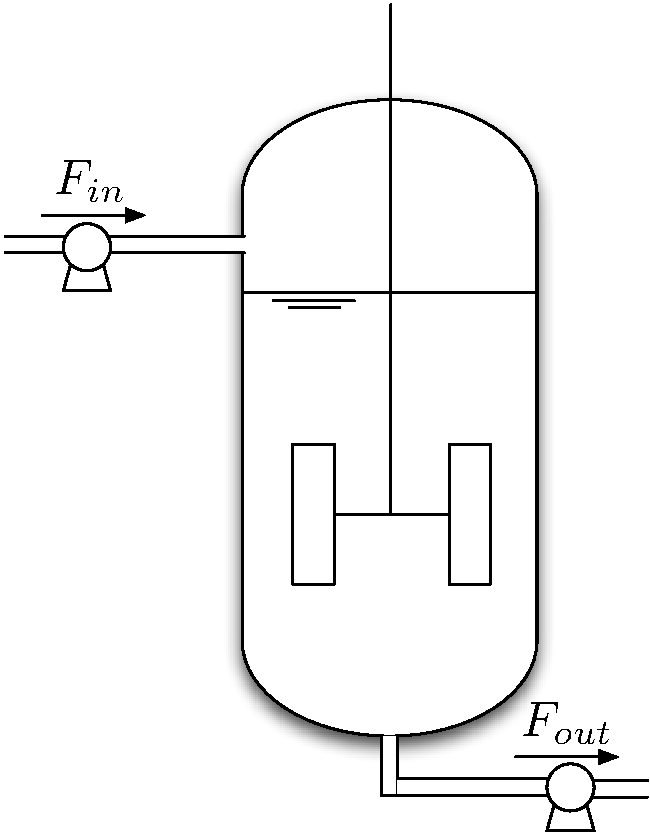
\includegraphics[height=6cm]{CSTR2} 
   \caption{Réacteur à volume variable}
   \label{Fig:CSTR2}
\end{figure}
L'équation matricielle de bilan massique des différentes espèces s'écrit
maintenant comme suit~:
$$
\frac{d}{dt} (xV) = Cr(x)V - F_{out}x + F_{in}x^{in}.
$$
Le volume du milieu réactionnel peut varier si les débits d'alimentation et de
soutirage sont différents. Les variations de volume sont décrites par l'équation de
bilan volumétrique~:
$$
\dot V = F_{in} -F_{out}.
$$
Si les deux débits volumétriques $F_{in}$ et $F_{out}$ sont
choisis comme variables d'entrée $u_1$ et $u_2$, on obtient le modèle d'état
suivant~: 
\begin{equation*} \begin{split}
\dot x &= Cr(x) + \frac{u_1}{x_{n+1}} (x^{in} - x), \\
\dot x_{n+1} &= u_1 - u_2,
\end{split} \end{equation*}
avec la variable d'état supplémentaire $x_{n+1}$ désignant le volume $V$.

Il est intéressant de choisir les débits par unité de volume $u_1 =
F_{in}/V$ et $u_2 = F_{out}/V$ comme variables d'entrée. Dans ce cas, le modèle
d'état s'écrit
\begin{equation*} \begin{split}
\dot x = Cr(x) + u_1(x^{in} - x), \\
\dot x_{n+1}= (u_1 - u_2)x_{n+1}.
\end{split} \end{equation*}
La première de ces deux équations décrit l'évolution de la
composition du réacteur. Elle est indépendante de $u_2$ et $x_{n+1}$ et elle est
identique à celle que nous avions obtenue pour un réacteur à volume constant
(\ref{CSTR}). 

\subsection{Réacteurs non-isothermes}

La vitesse d'une réaction chimique dépend aussi de la
température du milieu réactionnel. Jusqu'ici nous n'avons pas
pris cette dépendance en compte dans la modélisation : nous
avons implicitement supposé la température régulée à une
température parfaitement constante. En l'absence d'une telle
régulation, c'est la constante de vitesse qui dépend de la
température et la forme générale de la vitesse de la j-ième
réaction s'écrit
$$
r_j(x,T) = k_j(T)\rho_j(x)
$$
où $T$ désigne la température (en Kelvin) du milieu
réactionnel et la fonction $\rho_j(x)$ satisfait les conditions de
l'hypothèse (\ref{cond1})-(\ref{cond2}). La fonction $k_j(T)$ est
positive, bornée et $k_j(0) = 0$. Un exemple typique est donné
par la {\it loi d'Arrhenius} représentée à la figure
\ref{Fig:arrhenius}~: \eqnn
k_j(T) = k_{0j}exp(-\frac{E_j}{RT})
\eeqnn
\begin{figure}[htbp] 
   \centering
   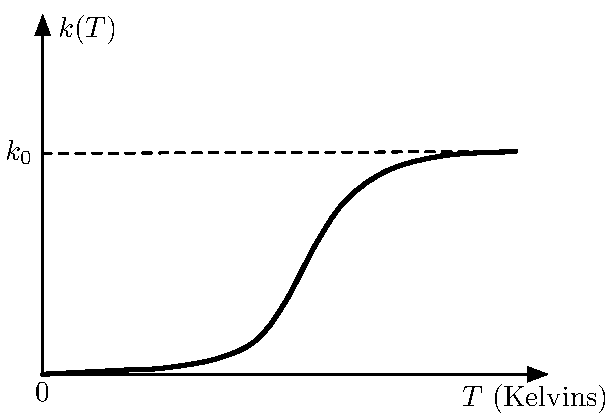
\includegraphics[width=8cm]{arrhenius} 
   \caption{Loi d'Arrhenius}
   \label{Fig:arrhenius}
\end{figure}
où $k_{0j}$ est une constante, $E_j$ l'énergie d'activation de la
réaction et $R$ la constante de Boltzmann. C'est une fonction
monotone croissante et bornée de la température. Dans
certaines applications (notamment en biotechnologie) la
fonction $k_j$ peut aussi être non monotone.

Le modèle d'état d'un réacteur non isotherme est obtenu en
ajoutant une équation de bilan énergétique aux équations de
bilan massique et volumique. A titre d'exemple, considérons un
réacteur continu muni d'un échangeur de chaleur.
L'équation de bilan énergétique s'écrit comme suit~:
$$
\delta c_p V\dot T = (\sum_{j=1}^{m}\Delta H_j r_j(x,T))V +
\delta c_p F_{in} (T_{in} - T) + Q
$$
où $\delta$ représente la densité du milieu réactionnel, $c_p$ la chaleur
spécifique, $\Delta H_j$ la chaleur de réaction, $T_{in}$ la
température du flux d'alimentation et $Q$ le flux de
chaleur échangé. Si on suppose que les paramètres $\delta$,
$c_p$ et $\Delta H_j$ sont constants, on obtient une équation
de bilan thermique~: 
$$ 
\dot T = \sum_{j=1}^{m} h_j r_j(x,T) +
d(T_{in} - T) + q
$$
où $h_j = \Delta H_j/c_p\delta V$ est la chaleur spécifique de
réaction, $d = F_{in}/V$ est le taux de dilution et $q =
Q/c_p \delta V$.

Les paramètres $h_j$ peuvent être positifs ou négatifs. Si
$h_j$ est négatif, la réaction en endothermique : elle
consomme de la chaleur qui est apportée dans le réacteur par
l'échangeur de chaleur. Si $h_j$ est positif, la réaction est
exothermique : elle génère de la chaleur dans le réacteur qui
doit être refroidi par l'échangeur de chaleur.

Le flux spécifique de chaleur échangée $q$ est lui même
fonction de la température $T$. Un modèle simple 
exprime que $q$ est proportionnel à la différence entre la
température du réacteur $T$ et la température d'entrée de
l'échangeur $T_w$~:
$$ q = e(T_w - T). $$
Dans ce cas, le modèle d'état global du réacteur s'écrit~:
\begin{equation*} \begin{split}
\dot x &= Cr(x) + d(x^{in} - x), \\
\dot x_{n+1} &= h^T r(x) + d(T_{in} - x_{n+1}) + e(T_w - x_{n+1}).
\end{split} \end{equation*}
avec la variable d'état supplémentaire $x_{n+1}$ désignant la
température $T$. Comme variables d'entrée, on peut choisir
par exemple le taux de dilution $d$ et le coefficient de
transfert thermique $e$ qui est proportionnel au débit de
l'échangeur de chaleur.

\section{Les systèmes écologiques} 

Le formalisme réactionnel et le
modèle d'état (\ref{sysrea}) conviennent aussi pour la description
d'une classe importante de systèmes écologiques (ou écosystèmes) dans
lesquels des populations d'organismes vivants (végétaux ou animaux) se
partagent un même habitat. 

Le modèle mathématique d'un écosystème se présente comme un cas
particulier de système réactionnel dans lequel~:
\begin{itemize}
\item le réseau réactionnel décrit les interactions entre espèces :
consommation de ressources inertes, pâturage sur des ressources
végétales, prédation, etc.  Les réactions sont nécessairement
autocatalytiques. 
\item les flux d'entrée représentent la fourniture de ressources au
système par des agents extérieurs et l'immigration de certaines espèces.
\item les flux de sortie représentent l'émigration des espèces vers
l'extérieur, la capture par des agents extérieurs (chasse, pêche, récolte,
cueillette, \dots) ou simplement la mortalité naturelle des espèces.
\end{itemize}

Nous commençons par un exemple simple.

\begin{exemple}{\bf \em Des algues dans la lagune}

Un nutriment organique provenant par exemple d'eaux ménagères
résiduaires ou de fertilisants agricoles est déversé dans une lagune. Une
population d'algues unicellulaires flottantes (phytoplancton) se développe
à la surface de l'eau en se nourrissant de ce nutriment. Cette situation peut
être schématisée par la réaction~:
\eqn
kY \longrightarrow X. \label{reacrois}
\eeqn
qui exprime que, dans le mécanisme de croissance des algues, le nutriment
$Y$ est transformé en matière vivante (ou biomasse) $X$ avec un
rendement $k^{-1}$. Comme tous les êtres vivants, les algues de la lagune
peuvent aussi mourir.

La lagune peut dès lors être considérée comme un vaste réacteur qui
transforme un réactif $Y$ (le nutriment) en un produit $X$ (la
biomasse). Le réacteur est alimenté par un flux entrant de réactif (le
nutriment déversé dans la lagune) tandis que la mortalité provoque un flux
sortant de produit. Sous une hypothèse
d'homogénéité spatiale, la dynamique de ce réacteur est décrite par
le modèle d'état
\begin{equation} \begin{split} \label{lagune}
\dot y &= -kr(x,y) + v, \\
\dot x &= r(x,y) - dx.
\end{split} \end{equation}
où $y$ représente la concentration en nutriment, $x$ la densité de la
population d'algues, $v$ le débit (par unité de volume) d'alimentation de la
lagune en nutriment, $dx$ la mortalité supposée proportionnelle à la
densité de population (le coefficient $d$ est le taux spécifique de
mortalité) et $r(x,y)$ la vitesse de réaction, c'est-à-dire ici la vitesse
de croissance des algues. \qed
\end{exemple}
D'un point de vue plus général, la réaction (\ref{reacrois}) peut
représenter la croissance d'une population quelconque d'organismes vivants
(végétaux ou animaux) $X$ qui, dans un habitat déterminé, consomme
une ressource alimentaire $Y$. Cette ressource alimentaire peut être de
la matière inerte (organique ou inorganique) comme dans l'exemple
ci-dessus. Elle peut aussi être une autre espèce vivante (végétale ou animale) : on parle
alors d'un modèle {\em proie - prédateur} dans lequel l'espèce ressource
$Y$ est la proie et l'espèce consommatrice $X$ est le prédateur.
D'évidence, cette réaction de croissance est autocatalytique puisque $X$
représente nécessairement une population d'êtres vivants autoreproducteurs~: 
\eqnn
kY \cata{X} X.
\eeqnn
Il est dès lors naturel de considérer que la vitesse de croissance est
proportionnelle à la densité de la population prédatrice et de représenter
la fonction $r(x,y)$ par un modèle de la forme~:
\eqnn
r(x,y) \teq \mu(x,y)x
\eeqnn
où la fonction $\mu(x,y)$ est appelée {\em vitesse spécifique de
croissance}. Cette fonction doit être définie de sorte que la vitesse de
réaction vérifie les conditions (\ref{cond1}) - (\ref{cond2}), c'est-à-dire~:
\begin{itemize}
\item $\mu(x,y)$ est une fonction positive définie sur l'orthant positif~:
\eqnn
\mu(x,y) \geq 0 \hh \hh \forall (x,y) \in \mathbb{R}_{+}^{2}.
\eeqnn
\item $\mu(x,0) = 0$ : il ne peut y avoir de croissance en l'absence de
ressource alimentaire.
\end{itemize}
La vitesse spécifique de croissance peut dépendre de nombreux facteurs
environnementaux. Deux effets non linéaires typiques sont l'effet de
{\em satiété} et l'effet de {\em surpopulation}.
\begin{description}
\item[Effet de satiété :] Lorsque la ressource alimentaire est rare, on
observe géné- ralement que la vitesse spécifique de croissance est une
fonction croissante de la quantité de ressource disponible. Il existe
cependant une limite physiologique à la vitesse de consommation
de la ressource et donc à la vitesse de croissance. Ceci se
modélise simplement en adoptant pour $\mu(x,y)$ une fonction
croissante saturée par rapport à $y$, telle que la vitesse de croissance
devient indépendante de $y$ au delà d'une concentration critique
$y_{c}$~: 
\eqnn
\frac{\partial \mu(x,y)}{\partial y} \geq 0, \hspace{1cm}
\mu(x,y) = \mu(x,y_{c}) \hh \hh \forall \hh y \geq y_{c}.
\eeqnn
\item[Effet de surpopulation :] Même quand la ressource alimentaire est
surabondante, la densité de la population est généralement limitée par
l'espace disponible. Ceci se modélise en imposant que la vitesse spécifique de
croissance $\mu(x,y)$ soit une fonction décroissante de la densité $x$
qui devient nulle quand la population atteint une valeur maximale $x_{m}$~:
 \eqnn
\frac{\partial \mu(x,y)}{\partial x} \leq 0, \hspace{1cm}
\mu(x,y) = 0 \hh \hh \forall \hh x \geq x_{m}.
\eeqnn
\end{description}

\begin{exemple}{\bf Le modèle de Contois.}

C'est un modèle classique de vitesse spécifique utilisé
pour décrire la croissance de populations de micro-organismes~:
\eqnn
\mu(x,y) = \frac{\mu_0 y}{y + Kx}.
\eeqnn
On observe que ce modèle est bien une fonction croissante bornée de $y$
(identique, à $x$ fixé, au modèle de Michaelis-Menten) et
décroissante (hyperbolique) de $x$. Cependant, les concentrations limites
de satiété $y_{c}$ et de surpopulation $x_{m}$ sont rejetées à l'infini.  \qed
\end{exemple}

\begin{exemple}{\bf Le modèle logistique}

Il est courant d'adopter pour la vitesse spécifique de croissance une
structure multiplicative de la forme~:
\eqnn
\mu(x,y) = \sigma(y)\phi(x).
\eeqnn
Cette structure permet de modéliser séparément les effets de satiété et
de surpopulation, par exemple de la manière suivante~:
\begin{equation*} \begin{split} \sigma(y) &= \left\{\begin{array}{ll}
\alpha y & \forall y \leq y_{c} \\ \alpha y_{c} & \forall y \geq y_{c} \end{array} \right.\\ \\
\phi(x) &= 
\left\{ \begin{array}{ll} (1 - \frac{x}{x_{m}}) & \forall x \leq x_{m} \\ 0  & \forall x \geq x_{m}
\end{array} \right.
\end{split} \end{equation*}
On observe que les fonctions $\sigma$ et $\phi$ sont linéaires et
saturées (voir figure  \ref{Fig:logistic}).
\begin{figure}[htbp] 
   \centering
   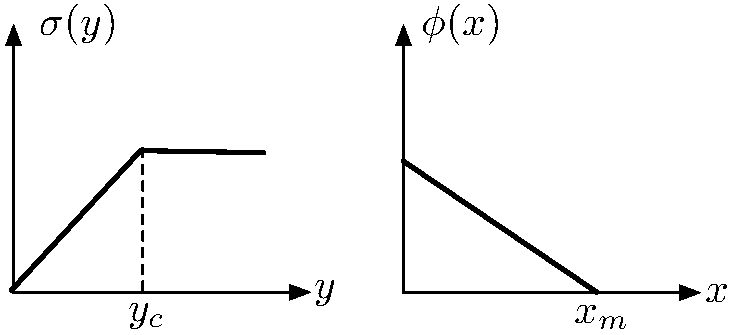
\includegraphics[height=5cm]{logistic} 
   \caption{Vitesse spécifique de croissance du modèle logistique}
   \label{Fig:logistic}
\end{figure}
Avec ces définitions, le modèle proie-prédateur
(\ref{lagune}) s'écrit, lorsque $y \leq y_{c}$ et $x \leq x_{m}$,
\begin{equation*} \begin{split}
\dot y &= -k\alpha xy(1 - \frac{x}{x_{m}}) + v, \\
\dot x &= \alpha xy(1 - \frac{x}{x_{m}}) - dx.
\end{split} \end{equation*}
Par contre, quand la ressource alimentaire est fournie au système en
quantité suffisante pour en maintenir la concentration au dessus de sa
valeur critique ($y(t) \geq y_{c} \hh \forall t$), alors la dynamique de
la population prédatrice devient {\em indépendante de la quantité de
ressource alimentaire disponible} et s'écrit simplement~:
\eqn
\dot x = \sigma_{c}x(1 - \frac{x}{x_{m}}) - dx  \label{logis}
\eeqn
où $\sigma_c = \alpha y_c$. La fonction $\phi(x) = (1 - x/x_{m})$ est généralement
dénommée {\em modèle logistique} dans la littérature. Par extension, le
modèle (\ref{logis}) est appelé modèle logistique de croissance d'une
population sur une ressource alimentaire non limitante.   \qed
\end{exemple}

Nous avons considéré jusqu'ici un modèle simple ne faisant intervenir que
deux espèces $X$ et $Y$. Cette description s'étend sans difficulté à
des écosystèmes plus complexes dans lesquels plusieurs espèces
biologiques, végétales ou animales, peuvent coexister et interagir au sein
d'un même habitat. Voici un exemple.

\begin{exemple} {\bf Un écosystème aquatique}

Un écosystème aquatique, comme tout système écologique naturel, est
géné-ralement caractérisé par la cohabitation de trois types
d'espèces biologiques : des espèces végétales, des espèces
animales herbivores et des espèces animales carnivores.  
\begin{figure}[htbp] 
   \centering
   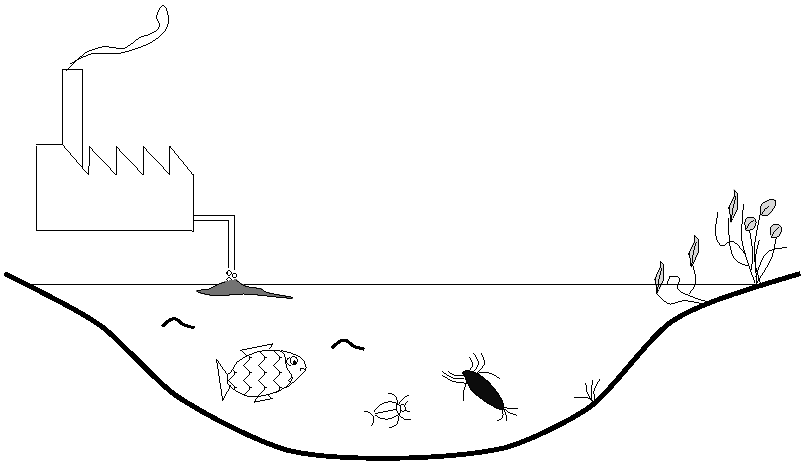
\includegraphics[height=5cm]{aquatic} 
   \caption{Ecosystème aquatique}
   \label{Fig:aquatic}
\end{figure}
A titre d'exemple, considérons un étang (voir figure
\ref{Fig:aquatic}) dans lequel est déversé un nutriment organique $X_1$.
Un population d'algues (phytoplancton) $X_2$
se développe par consommation de ce nutriment.  Une population de petits
crustacés herbivores $X_3$ p\^ature sur le phytoplancton qui constitue sa
ressource alimentaire principale. Une population de poissons carnivores $X_4$
assure son développement et sa subsistance par la consommation des
crustacés. La respiration animale consomme l'oxygène $X_5$ en solution
dans l'eau produit par la photosynthèse. Cette description est
schématisée par le réseau réactionnel suivant~:
\eqnn
c_1X_1 &\cata{X_2}& X_2 + c_4X_5, \\
c_2X_2 + c_5X_5 &\cata{X_3}& X_3, \\
c_3X_3 + c_6X_5 &\cata{X_4}& X_4. 
\eeqnn
Un modèle d'état du système est établi sous les hypothèses de
modélisation et avec les notations suivantes.
\begin{itemize}
\item Le nutriment organique est déversé avec un débit par unité de
volume $v$.
\item les trois espèces biologiques sont sujettes à une mortalité
naturelle. Les coefficients de mortalité sont notés $d_i, i = 2,3,4$.
\item Les poissons sont de plus l'objet d'une pêche dont l'intensité est
proportionnelle à la densité de la population. Le coefficient de
proportionnalité est noté $d_1$. 
\item La cinétique de croissance des
algues est décrite par le modèle logistique, avec une dépendance de
Michaelis Menten par rapport à la concentration en nutriment. 
\item Les deux
cinétiques de croissance des populations animales sont décrites par le
modèle de Contois avec une dépendance de Michaelis Menten par rapport
à la concentration en oxygène dissous. 
\end{itemize} 
Le modèle d'état de
cet écosystème aquatique s'écrit~: 
\begin{equation*} \begin{split}
\bma{c}  \dot x_1 \\ \dot x_2 \\
\dot x_3 \\ \dot x_4 \\ \dot x_5 \ema &= \bma{ccc} -c_1 & 0 & 0\\ 1 & -c_2
& 0 \\ 0 & 1 & -c_3 \\ 0 & 0 & 1 \\ c_4 & -c_5 & -c_6 \ema \bma{c}
\frac{{\textstyle \mu_1 x_1 x_2}}{{\textstyle x_1 + K_1}}(1 -
\frac{{\textstyle x_2}}{{\textstyle x_{2c}}}) \\ 
\\
\frac{{\textstyle \mu_2 x_2 x_3}}{{\textstyle x_2 + K_2x_3}}  \frac{{\textstyle
x_5}}{{\textstyle x_5 +K_4}} \\
\\
\frac{{\textstyle \mu_3 x_3 x_4}}{{\textstyle x_3 + K_3x_4}} \frac{{\textstyle
x_5}}{{\textstyle x_5 +K_5}}
\ema 
\\ & \\&- \bma{ccccc} 0 & 0 & 0 &
0 & 0 \\ 0 & d_2 & 0 & 0 & 0 \\0 & 0 & d_3 & 0 & 0  \\0 & 0 & 0 & d_1 + d_4 & 0
\\0 & 0 & 0 & 0 & 0
\ema \bma{c} x_1 \\  x_2 \\  x_3 \\  x_4 \\ x_5 \ema + \bma{c} v \\ 0  \\ 0 \\
0 \\ 0 \ema.    
\end{split} \end{equation*}
Les variables d'état
$x_2,x_3,x_4$ désignent les densités des trois populations biologiques
tandis que $x_1$ et $x_5$ désignent respectivement les concentrations en
nutriment et en oxygène dissous. \qed
\end{exemple}
 
\section{Exercices}

\begin{exercice}{\bf \em Un procédé chimique}

Une installation de génie chimique est représentée à la figure
\ref{Fig:genchim}. Une réaction réversible $A+B \leftrightarrow C$, obéissant
à la loi d'action des masses, se déroule dans le réacteur.
\begin{figure}[htbp] 
   \centering
   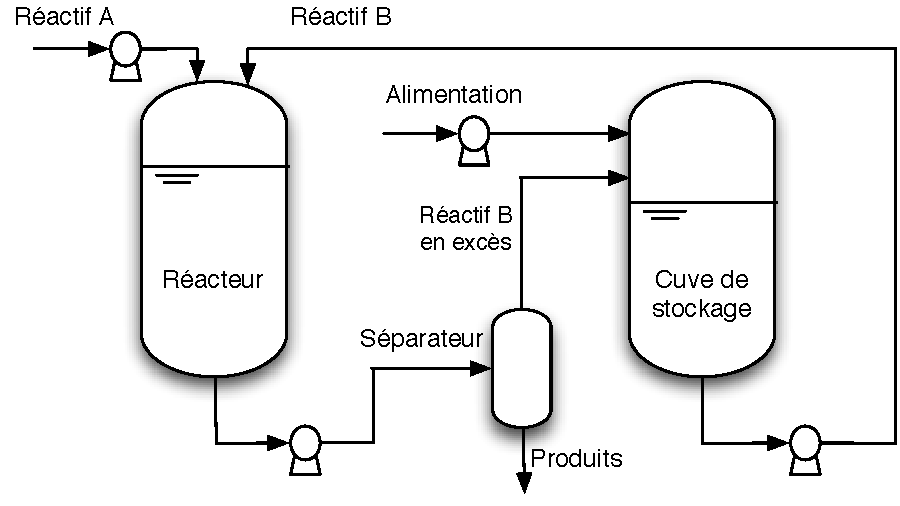
\includegraphics[height=6cm]{genchim} 
   \caption{Un procédé chimique}
   \label{Fig:genchim}
\end{figure}
 Le séparateur est
supposé opérer une séparation parfaite et instantanée des trois
espèces chimiques. Le réactif $B$ est recyclé via une cuve de
stockage. Le réactif $A$ et le produit $C$ sont soutirés du système.
Proposer un modèle d'état du système. \qed
\end{exercice}
\vv

\begin{exercice}{\bf \em Réacteur avec alimentations séparées}

Nous avons considéré dans ce chapitre que les différentes espèces qui alimentent un
réacteur sont fournies ensemble par une canalisation unique (voir par exemple la
figure \ref{Fig:CSTR}). Un tel dispositif peut avoir l'inconvénient de voir les
réactions débuter dans la canalisation d'amenée avant d'atteindre le réacteur. Cet
inconvénient est évité si les réactifs sont introduits dans le réacteur par des
canalisations séparées. Reconsidérons l'exemple \ref{exempleCSTR} avec des alimentations séparées pour
les deux réactifs $X_1$ et $X_2$ (voir figure \ref{Fig:CSTRsepar})~:
\begin{figure}[htbp] 
  \centering
   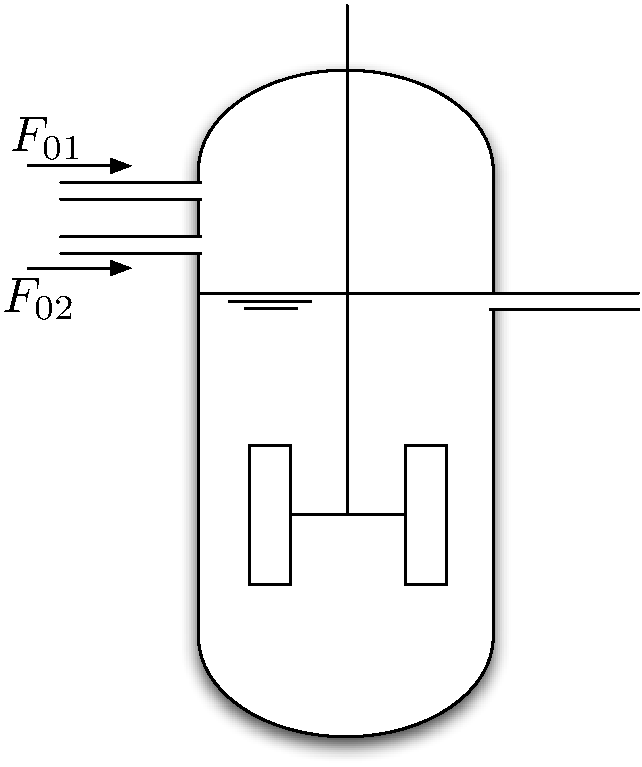
\includegraphics[height=6cm]{CSTRsepar} 
   \caption{Réacteur continu avec alimentations séparées}
   \label{Fig:CSTRsepar}
\end{figure}
\begin{enumerate}
\item Etablir un modèle d'état du système si les variables d'entrée sont les deux débits volumique d'alimentation $F_{01}$ et $F_{02}$.
\item Un cas particulier intéressant est celui ou le réacteur
est alimenté à débit volumique total constant ($F_{01} + F_{02} =$ constante).
Seule la composition de l'alimentation est variable. En pratique cela peut être
réalisé en ajustant complémentairement les deux débits $F_{01}$ et $F_{02}$
avec une vanne à quatre voies (voir figure \ref{Fig:vanne4voies}) de manière
que leur somme soit constante.  
\begin{figure}[htbp] 
   \centering
   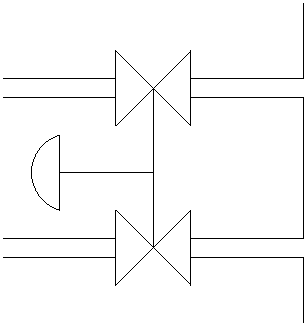
\includegraphics[height=4cm]{vanne4voies} 
   \caption{Alimentations séparées avec vanne à quatre voies}
   \label{Fig:vanne4voies}
\end{figure}
On choisit le débit $F_{01}$
comme unique variable d'entrée et on définit le taux de dilution constant $d =
(F_{01} + F_{02})/V$. Etablir le modèle d'état du système et montrer qu'il s'écrit sous la forme (\ref{sysrea}). \qed
\end{enumerate}
\end{exercice}
\vv

\newpage
\begin{exercice}{\bf \em Réactifs et produits gazeux}

Le modèle d'état (\ref{CSTR}) d'un réacteur continu parfaitement mélangé
peut être étendu au cas de réactifs ou de produits gazeux. Supposons tout
d'abord que le réacteur soit alimenté par un réactif $X$ sous forme gazeuse
(par exemple de l'oxygène) avec un débit massique $Q_{in}$ (voir figure
\ref{Fig:CSTRgaz}).
\begin{figure}[htbp] 
   \centering
   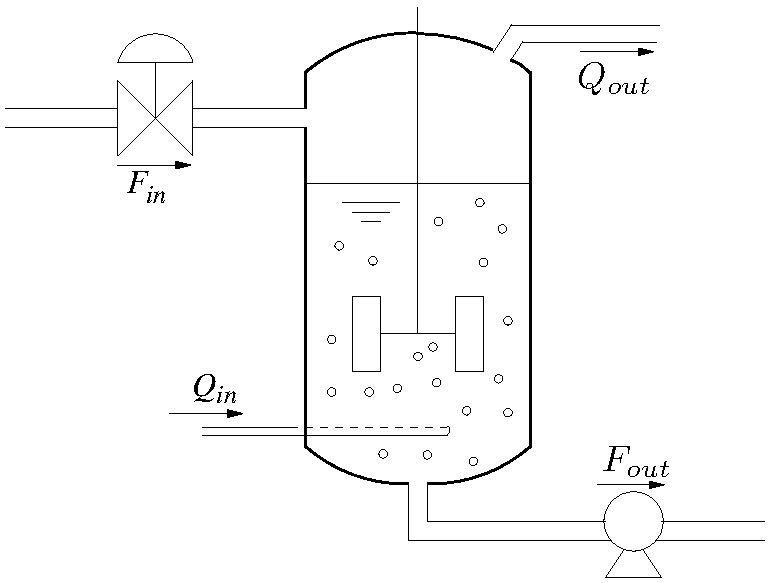
\includegraphics[height=6cm]{CSTRgaz} 
   \caption{Réacteur avec réactifs et produits gazeux}
   \label{Fig:CSTRgaz}
\end{figure}
Le réactif barbote dans le milieu liquide où il est partiellement dissous. L'excès de
réactif non-dissous s'échappe librement du réacteur sous forme gazeuse avec un
débit massique $Q_{out}$. La quantité de réactif mise en solution par unité
de temps est donc $Q_{in} - Q_{out}$. En se basant sur la loi de Henry et en
négligeant la dynamique du transfert gaz-liquide, on peut modéliser cette
quantité comme étant proportionnelle au débit gazeux d'alimentation d'une part
et au déficit de saturation d'autre part~:
\eqnn
Q_{in} - Q_{out} = aQ_{in}(x^{sat} - x)
\eeqnn
où $x$ désigne la concentration de l'espèce $X$ en solution et $x^{sat}$ la
concentration de saturation de cette même espèce dans la phase liquide.

Considérons maintenant qu'un produit de réaction $X$ (par exemple du $CO_2$)
formé en solution est gazéifiable. Il s'échappe du milieu réactionnel avec un débit
massique $Q_{out}$. Sous une hypothèse d'équilibre entre les phases liquide et
gazeuse, on peut considérer que ce débit est proportionnel à la concentration du
produit $X$	en solution dans le milieu réactionnel~:
\eqnn
Q_{out} = dx
\eeqnn
\begin{enumerate}
\item Comme dans l'exemple \ref{exempleCSTR}, considérons un réacteur
continu  dans lequel
 les deux réactions (\ref{exa})-(\ref{exb})
se déroulent simultanément dans la phase liquide avec les cinétiques
(\ref{cin}).  Cette fois, nous supposons cependant que le
réactif $X_2$ et le produit $X_4$ sont sous forme gazeuse. 
On demande d'établir le modèle d'état du système sous les hypothèses de modélisation suivantes~: 
\begin{itemize} 
\item Le réacteur est alimenté par le réactif initial $X_1$ en
solution avec un débit volumétrique $F_{in}$ et une
concentration d'alimentation $x_1^{in}$. 
\item Le réactif $X_2$ est injecté dans le réacteur sous forme gazeuse.
  La quantité de réactif $X_2$ mise en
solution par unité de temps est notée $aQ_{in}(x_2^{sat} - x_2)$.
\item Les produits $X_3$ et $X_4$ sont
formés en solution dans le milieu réactionnel. Le produit $X_4$ est
gazéifiable et s'échappe du réacteur avec un débit gazeux $dx_4$.
\end{itemize}
\item Si les variables d'entrée sont le débit volumétrique d'alimentation liquide par unité de
volume de milieu réactionnel $u_1 = F_{in}/V$ et le débit massique d'alimentation
gazeuse par unité de volume de milieu réactionnel $u_2 = Q_{in}/V$, montrer
que le modèle d'état possède la structure (\ref{sysrea}). \qed
\end{enumerate}
\end{exercice}
\vv

\begin{exercice}{\bf \em Une réacteur biochimique}

Un réacteur biochimique fonctionnant en mode CSTR met en jeu trois
espèces : une population bactérienne $X_1$, du glucose $X_2$,
et du lactose $X_3$.\\

La dynamique du réacteur est décrite par le modèle d'état suivant
($x_i$ désigne la concentration de l'espèce $X_i$): 
\begin{equation*} \begin{split}
\dot x_1 &= x_1x_2-ux_1,\\
\dot x_2 &= -x_1x_2 +x_1x_3 -ux_2,\\
\dot x_3 &= -x_1x_3 +u(c-x_3) \;\;\;\; c>0. 
\end{split} \end{equation*}

\begin{enumerate}
\item Quel est le schéma réactionnel ?
\item L'entrée $u$ est positive :  $u>0$.  Que représente-t-elle physiquement ?
\item Montrer que le système est positif. \qed
\end{enumerate}
\end{exercice}
\vv

\begin{exercice}{\bf \em Des coccinelles et des pucerons}

Montrer que le système (\ref{coc}) du chapitre 1 modélisant l'interaction entre les populations de coccinelles et de pucerons est un système réactionnel. \qed
\end{exercice}
\vv

\begin{exercice}{\bf \em Une station d'épuration biologique aérobie}

Une station d'épuration biologique aérobie est schématisée à la
figure \ref{Fig:epurat}.
\begin{figure}[htbp] 
   \centering
   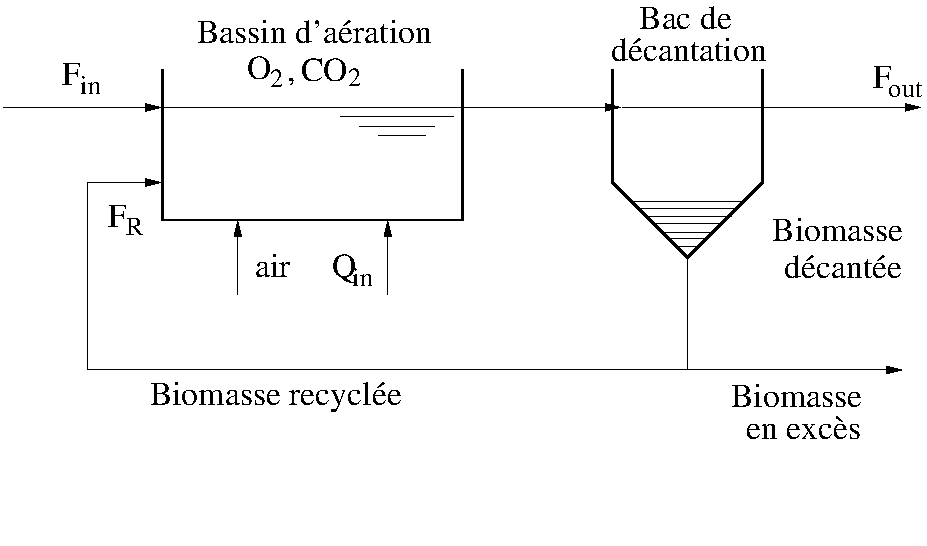
\includegraphics[width=11cm]{epurat} 
   \caption{Station d'épuration biologique aérobie}
   \label{Fig:epurat}
\end{figure}
Le bassin d'aération est alimenté par des eaux  usées
(débit
$F_{in}$) contenant un substrat organique polluant  (concentration $S$). 
Ce substrat organique est dégradé par des microorganismes
(concentration $X$) aérobies.  Cette dégradation nécessite de
l'oxygène dissous dans l'eau (concentration $O$) et produit du dioxyde
de carbone (concentration
$C$) sous forme dissoute mais qui se gazéifie aisément et sort du
système sous forme gazeuse.  L'oxygène dissout est fourni par un
système d'aération (débit d'air $Q_{in}$).  On fait l'hypothèse que
les dynamiques de transfert entre phase gazeuse et phase liquide sont
négligeables (instantanées).

La sortie du bassin d'aération est connectée à un bac de
sédimentation (décantation) où la biomasse (c'est à dire la masse 
des microorganismes) est séparée du reste.  L'eau clarifiée est
évacuée du système (débit $F_{out}$).  La biomasse est recyclée
vers le bassin d'aération (débit $F_R$).  Cependant, on prévoit la
possibilité d'éliminer la biomasse en excès (débit $F_S$).  Les
niveaux dans le bassin d'aération et dans le décanteur sont
supposés constants.  Le bassin d'aération est supposé parfaitement
mélangé.  Le bassin de décantation (qui ne peut être
parfaitement mélangé !) est modélisé par deux réservoirs
(compartiments) parfaitement mélangés (un pour l'eau clarifiée, un
pour la biomasse décantée).  On suppose aussi qu'il n'y a aucune
réaction biologique dans le décanteur. On demande d'établir un modèle d'état du système. \qed
\end{exercice}
\vv

\begin{exercice}{\bf \em Un système non conservatif}

Soit le réseau réactionnel suivant~:
\begin{equation*} \begin{split} 
X_1   &\longrightarrow X_2 + X_3 \\
X_3 &\longrightarrow 2X_1 + X_4
\end{split} \end{equation*}
\begin{enumerate}
\item Etablir le modèle d'état d'un système réactionnel fermé
sous les hypothèses de modélisation suivantes : principe d'action des
masses pour la première réaction avec une vitesse d'ordre 2
par rapport à tous les réactifs, cinétique de Michaelis-Menten pour
la deuxième réaction avec inhibition hyperbolique par $X_2$.
\item Montrer que le système n'est pas conservatif. Donner une
justification physique.
\item Montrer qu'il suffit d'ajouter un réactif initial dans la première 
ou la deuxième réaction pour rendre le système conservatif. \qed
\end{enumerate}
\end{exercice}

\end{document}
  

